\documentclass[12pt]{article}
\usepackage{minted}
\usepackage{graphicx}
\usepackage{mathtools}
\usepackage{amsfonts}
\usepackage{tikz} 

\begin{document}
    \title{CS 559 Homework 3}
    \author{Stephen Szemis}
    \date{December 11, 2020}
    \maketitle

    I pledge my honor that I have abided by the Stevens honor system.

    \paragraph{Problem 1: K-Mean}
    \subparagraph{1.}
    \begin{verbatim}
    iteration :  1
    center of RED is [5.171 3.171]
    \end{verbatim}
    \subparagraph{2.}
    \begin{verbatim}
    iteration :  2
    center of GREEN is [5.3 4.0]
    \end{verbatim}
    \subparagraph{3.}
    \begin{verbatim}
    iteration :  3
    center of BLUE is [6.2   3.025]
    \end{verbatim}
    \subparagraph{4.}
    The centers converge after 2 iterations.
    
    \paragraph{Problem 2: K-Means and gradient descent}
    \subparagraph{1.}
    Starting with our loss function.
    \[
        L = \sum_{j=1}^{k} \sum_{x_i \in S_j} \parallel x_i - u_j \parallel ^ {2}
    \]
    We then take the gradient with respect to \(u_1\) in order to derive the update formula. Remember that since
    we are using batch gradient decent, we will make use of all of our data.
    \[
        \frac{\partial L}{\partial u_1} = \frac{\partial}{\partial u_1}
        \sum_{x_i \in S_j} \parallel x_i - u_1 \parallel ^ {2} +
        \sum_{x_i \in S_j} \parallel x_i - u_2 \parallel ^ {2} +
        \dots +
        \sum_{x_i \in S_j} \parallel x_i - u_i \parallel ^ {2}
    \]
    \[
        \frac{\partial L}{\partial u_1} =
        2\sum_{x_i \in S_j}  (x_i - u_1) +
        0 +
        \dots +
        0
    \]
    \[
        \frac{\partial L}{\partial u_1} =
        -2\sum_{x_i \in S_j}  (x_i - u_1)
    \]
    So the update rule is.
    \[
        \hat{\mu_1} = \mu_1 + 2 \epsilon \sum_{x_i \in S_j}  (x_i - u_1)
    \]
    \subparagraph{2.}
    This is very similar to batch gradient decent, except we now only use one piece of data randomly selected.
    The gradient is the same as before, but our update rule changes to.
    \[
        \hat{\mu_1} = \mu_1 + 2 \epsilon (x_i - u_1)
    \]
    For some \(x_i\) randomly selected at each update step.
    \subparagraph{3.}
    In order to create the standard update step, we need to rearrange our batch gradient decent update rule as follows.
    \[
        \hat{\mu_1} = \mu_1 + 2 \epsilon \sum_{x_i \in S_j}  (x_i - u_1)
    \]
    \[
        \hat{\mu_1} = \mu_1 + 2 \epsilon \left( \sum_{x_i \in S_j}  (x_i)  - (\parallel S_j \parallel) \mu_1 \right)
    \]
    Make \(\epsilon = \frac{1}{2 \parallel S_j \parallel}\) and we get.
    \[
        \hat{\mu_1} = \mu_1 + 2 \frac{1}{2 \parallel S_j \parallel} \left( \sum_{x_i \in S_j}  (x_i)  - (\parallel S_j \parallel) \mu_1 \right)
    \]
    Simplify:
    \[
        \hat{\mu_1} = \mu_1 - \mu_1 + \frac{1}{\parallel S_j \parallel}\sum_{x_i \in S_j}  (x_i)
    \]
    \[
        \hat{\mu_1} = \frac{1}{\parallel S_j \parallel}\sum_{x_i \in S_j}  (x_i)
    \]
    Which is the exact k-means update rule.

    \paragraph{Problem 3: Latent variable model and GMM}
    \subparagraph{1.}
    \[
        p(\mathbf{z}) = \prod_{k=1}^{K} \pi_{k}^{z_k}
    \]
    \[
        p(\mathbf{x} | \mathbf{z}) = \prod_{k=1}^{K} \mathcal{N} (\mathbf{x} | \mu_k, \Sigma_k)^{z_k}
    \]
    \subparagraph{2.}
    We notice that because \(z\) is using a 1-of-K representation, we can say that only 1 value of k in the above products will 
    be non-zero. Therefore\dots
    \[
        p(\mathbf{x}) = \sum_{\mathbf{z}} p(\mathbf{z}) p(\mathbf{x} | \mathbf{z}) =
        \sum_{k=1}^{K} \pi_{k} \mathcal{N} (\mathbf{x} | \mu_k, \Sigma_k)
    \]
    \subparagraph{3.}
    We can use the Expectation Maximization Algorithm in order to solve our latent variable model. This is different from k-means because
    it uses a soft assignment, that is, each data point is not associated uniquely with one cluster. Instead they are 
    associated with multiple clusters according to there posterior probabilities. This allows the Algorithm to be more accurate in some cases,
    however it can also be slower and harder to implement.

    \paragraph{Problem 4: Bayesian Network}
    \subparagraph{1.}
    The graph looks like the following.

    \begin{center}
        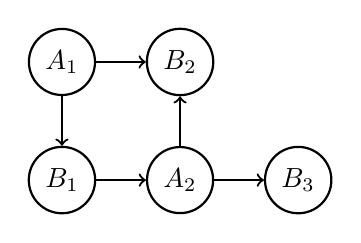
\begin{tikzpicture}[node distance={15mm}, thick, main/.style = {draw, circle}] 
        \node[main] (1) {\(A_1\)};
        \node[main] (2) [below of=1] {\(B_1\)};
        \node[main] (3) [right of=1] {\(B_2\)};
        \node[main] (4) [below of=3] {\(A_2\)};
        \node[main] (5) [right of=4] {\(B_3\)};
    
        \draw[->] (1) -- (2);
        \draw[->] (1) -- (3);
        \draw[->] (2) -- (4);
        \draw[->] (4) -- (3);
        \draw[->] (4) -- (5);
        \end{tikzpicture}
    \end{center}

    \subparagraph{2.}
    \[
        p(A_1, A_2, B_1, B_2, B_3) = p(B_3 | A_2) p(A_2 | B_1) p(B_1 | A_1) p(B_2 | A_1, A_2) p(A_1)
    \]
    \subparagraph{3.}
    We need one independent parameter in order to fully specify the joint probability. Since ultimately every is dependent on \(A_1\).

    \subparagraph{4.}
    In this example we will use this factorization.
    \[
        p(A_1, A_2, B_1, B_2, B_3) = p(B_3 | B_1) p(B_2 | B_1) p(B_1 | A_1, A_2) p(A_1) p(A_2)
    \]
    And therefore we need 2 independent parameters.

    \paragraph{Problem 5: Neural Network}
    \subparagraph{1.}
    You can view the full code at the end of this document. I had two sigmoid activated layers with a 
    hidden node number of 6. This gave okay results, but it seemed very dependent on the initial values of our
    weights. Often the model would be stuck in what seemed to be a steady state of some sort, unable to correctly
    "learn" from our data. I have a feeling this is because of the Sigmoid activation, which really isn't all that 
    good at distinguishing between multiple classes. It's good for a binary classification problem, but we had three 
    classes to learn. I ended up with accuracy in the area of 0.9. You can view the graphs of our accuracy below.
    \begin{center}
    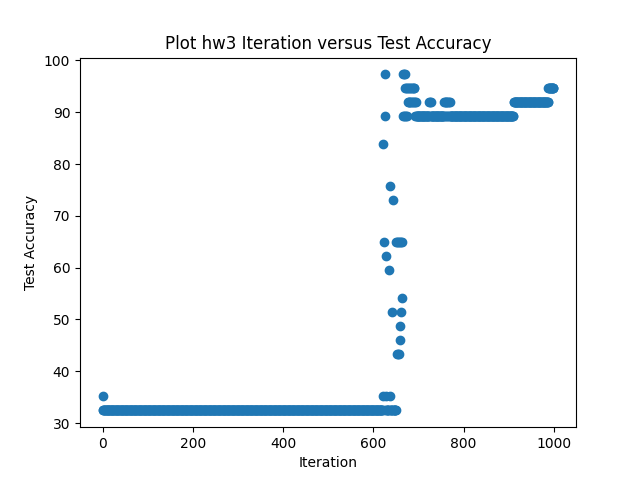
\includegraphics[width=5cm]{hw3_test.png}
    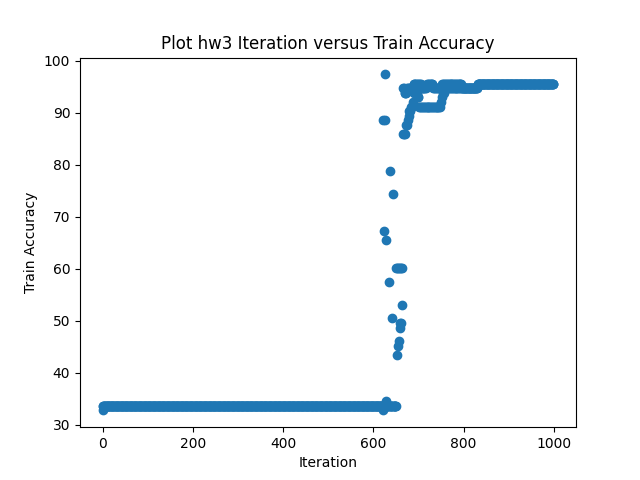
\includegraphics[width=5cm]{hw3_train.png}
    \end{center}

    \subparagraph{2.}
    I used Keras from tensorflow to create my learning network. I'll explain the reasoning behind my final code.
    First I used three different layers, a RELU layer with 32 nodes, another RELU layer with 
    16 nodes, and a softmax layer with 3 nodes. The RELU layers are mostly there to give "space" to learn. I found that
    adding more nodes did increase my accuracy up to a point, this seemed like a good number. I choose RELU because it's 
    easy to compute and it give the benefits of a linear activation layer without the issues of negative weights. The softmax
    layer simply gives a percent chance for our three classes. So it output a vector of probabilities that our input is either class A,
    B, or C. This is very helpful when doing multi-classification problems.

    We also use a keras function which turns our "class labels" into a binary vectors. So\dots
    \[
        0 => [1, 0, 0]
        1 => [0, 1, 0]
        2 => [0, 0, 1]
    \]

    This really just so that our keras function can easily map our final predictions easily.
    We got around 97 percent accuracy, so it's much MUCH better then my simple network.

    \paragraph{Code for part 1:}
    \inputminted{python}{Szemis_hw3_part1.py}

    \paragraph{Code for part 5:}
    \inputminted{python}{Szemis_hw3_part5.py}

\end{document}